%%%%%%%%%%%%%%%%%%%%%%%%%%%%%%%%%%%%%%%%%%%%%%%%%%%%%%%%%%%%%%%%%%%%%%%%%%%%%%%%
\chapter{Design and Implementation}
%%%%%%%%%%%%%%%%%%%%%%%%%%%%%%%%%%%%%%%%%%%%%%%%%%%%%%%%%%%%%%%%%%%%%%%%%%%%%%%%
\label{sec:design}

In this chapter we describe Landslide's implementation in detail. Section~\ref{sec:model} outlines the testing model on top of which Landslide's exploration mechanisms are built. Section~\ref{sec:components} describes the individual components within Landslide. Section~\ref{sec:techniques-bugs} describes Landslide's metrics for identifying bugs. Section~\ref{sec:techniques-por} describes how Landslide achieves effective state space reduction. Section~\ref{sec:techniques-feedback} describes the debugging feedback Landslide provides to the user when bugs are encountered.

\revision{
\section{Landslide's View of the World}
\label{sec:model}

Landslide's model for applying systematic exploration in kernel-space is comprised of four key points, which we overview here.

\subsection{Simulated Execution}
\label{sec:model-simics}

Landslide is implemented as a module for Simics\cite{simics}, a full-system x86 emulator. When running the kernel, Simics calls into Landslide once every time the kernel executes an instruction or performs a memory read or write. Landslide uses this information, in conjunction with the user-provided instrumentation, to maintain its internal representations of the state of the guest kernel.

Landslide makes use of Simics ``bookmarks'', a feature which enables checkpointing and restoring the execution state of the guest kernel, to implement backtracking when the end of each branch in the decision tree is reached.

\subsection{Timer-Driven Scheduling}
\label{sec:model-timer}

In this work, we focus specifically on nondeterministic scheduling driven by timer interrupts. Landslide assumes that timer interrupts are the only source of nondeterminism for the guest kernel, so controlling when they occur theoretically allows for complete control over the concurrent behaviour of the test case. In future work (Section~\ref{sec:future-drivers}), we may also address causes of non-determinism more complex than timer-driven thread scheduling, such as interrupts and data I/O from peripheral devices.

Landslide needs to impose some requirements on the guest kernel's scheduling behaviour, in order for its control over scheduling to work:

\begin{itemize}
	\item {\bf Timer ticks control ``runnable'' threads.} With the exception of a non-preemptible ``scheduler lock'', and yield-looping mutexes (both of which must be instrumented by the user), a thread's presence on the runqueue indicates that a finite number of timer interrupts in succession will eventually cause it to run.

	Landslide treats the sleep queue no differently from the runqueue when deciding which threads are runnable. The guest kernel will treat it differently, but since sleeping for a predetermined amount of time is never an appropriate way to solve race conditions, Landslide treats sleeping threads as notionally runnable. This fits directly into its model that runnable threads are ones that can be caused to run with a finite number of timer ticks in succession.
	\item {\bf No idling when progress can be made.} The kernel must not enter its idle loop (whether in an explicit idle thread or no) when the kernel is not truly idle. Landslide uses the idle loop to detect when a test begins/ends (test lifecycle tracking) and to detect when all threads in a test are wedged (bug detection).
\end{itemize}

Section~\ref{sec:components-inflight} gives more detail about how Landslide abstracts raw timer interrupts into the ability to cause arbitrary threads to run.

\subsection{False-Negative-Oriented Bug Detection}
\label{sec:model-bugs}

% A healthy dose of snark.
Without a formal specification of the internals of the guest kernel's implementation\cite{sel4}, it is impossible to identify both soundly and completely when a behaviour that constitutes a ``bug'' arises during a test case's execution.
Landslide's bug reporting is false-negative oriented, meaning that it does not check for suspicious behaviours that might indicate underlying bugs, so it may report that it found no bugs even if some existed. If Landslide does report a bug, though, it is almost certainly correct. Section~\ref{sec:techniques-bugs} details the conditions Landslide uses to identify when something has gone wrong.

\subsection{User-Assisted State Space Reduction}
\label{sec:model-user}

In addition to Dynamic Partial Order Reduction (DPOR) for automated state space reduction, Landslide relies on the user's guidance to help mitigate the possible combinatorial explosion of thread interleaving possibilities. This manifests in two ways:

\begin{itemize}
	\item {\bf Decision point selection.} Landslide provides an interface for the user to manually limit identification of decision points to only ``relevant'' modules of the kernel, thereby only generating thread interleavings around points within those modules.
	\item {\bf Memory conflict selection.} Landslide also provides a mechanism for ignoring shared memory conflicts on certain common data structures (especially those accessed in every thread transition, such as the scheduler queues), to enable DPOR to achieve greater reduction. Intuitively, this represents sacrificing the ability to find races around those data structures to make searching other components more feasible.
\end{itemize}

We advocate relying on the user for such information because the user need only understand the basics of their kernel design (which is difficult for Landslide to guess) while not knowing in advance what bugs are being looked for (which Landslide is able to provide). We claim that this combination of the user's knowledge and Landslide's testing mechanisms leads to an effective usage dynamic, in which the user ``steers'' Landslide towards focused search spaces that are more likely to find bugs.

The interfaces by which the user provides this information are documented in Section~\ref{sec:using-customise}.
}

\section{Components of Landslide}
\label{sec:components}

In this section we briefly describe each major component of Landslide.

\begin{figure}[h]
	\centering
	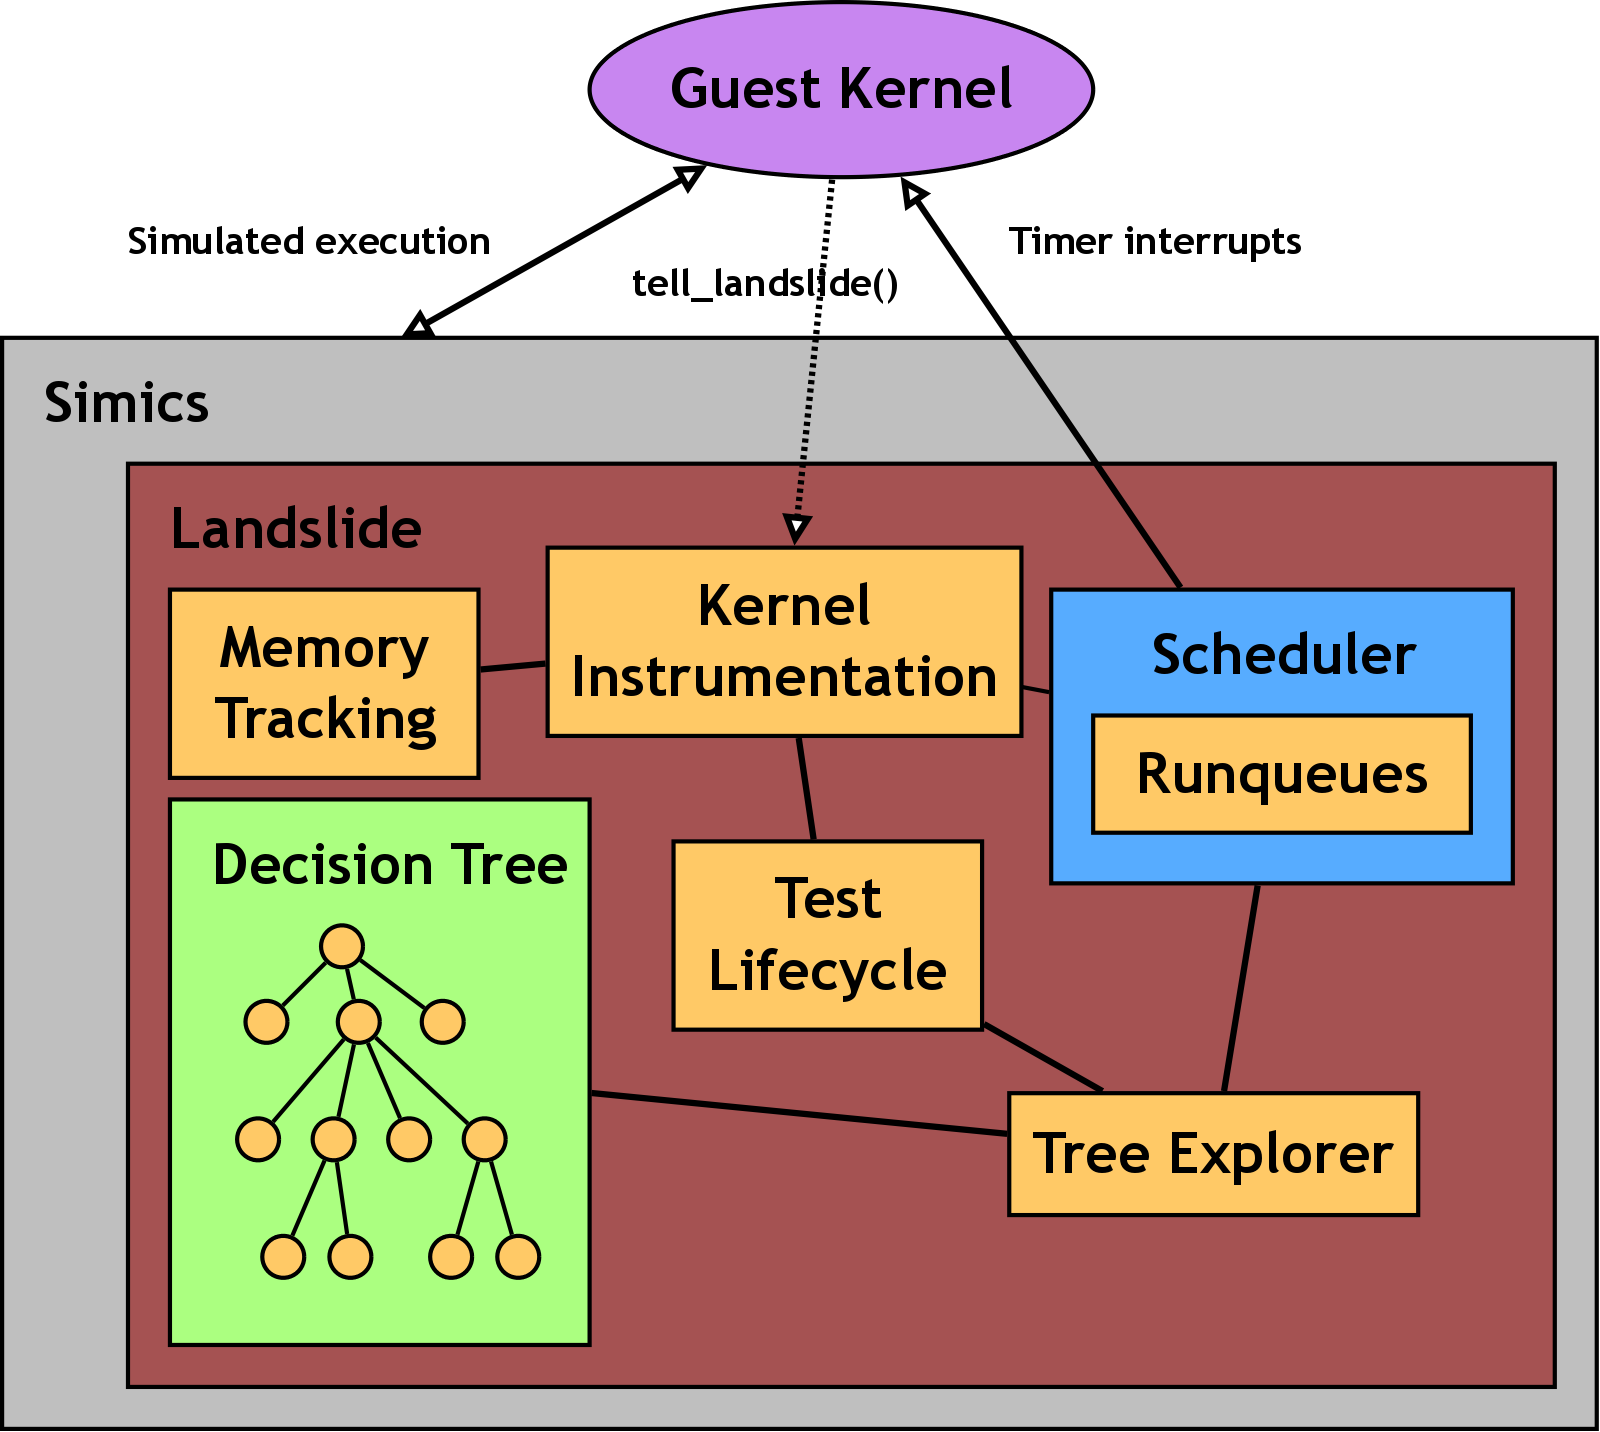
\includegraphics[width=0.75\textwidth]{landslide.png}
	\caption{A simple visualisation of Landslide and its components, and how they interact with the guest kernel.}
	\label{fig:landslide}
\end{figure}

\subsection{Kernel Instrumentation}
\label{sec:components-kern}

The kernel instrumentation serves as the glue between what the guest kernel is doing and Landslide's understanding of the guest kernel's state.

\begin{itemize}
	\item {\bf User-provided instrumentation.} Some parts of the kernel may be written in any number of ways, and hence require the user's assistance for Landslide to understand. The user-provided instrumentation, described in detail in Section~\ref{sec:using-instrumenting}, informs Landslide about thread-related lifecycle and scheduling events and the anatomy of the kernel's scheduler.
	\item {\bf Automatic instrumentation.} All Pebbles kernels have some things in common (largely due to the common starter code provided for the class project), and Landslide's build system is able to automatically instrument certain parts of the kernel. This instrumentation informs Landslide about the dynamic memory allocator, common library functions such as \texttt{panic}, and certain aspects of the kernel's executable format.
\end{itemize}

\subsection{Scheduling}
\label{sec:components-sched}

The Landslide scheduler is responsible for keeping track of which threads exist in the guest kernel: which are runnable at any given time, and when they are created and destroyed.

It maintains a ``mirror image'' of the guest kernel's scheduler state in the form of three queues, a pointer to the currently-running thread, and a pointer to the previously-running thread. The queues are the {\em runqueue}, containing the runnable threads, the {\em sleep queue}, containing threads which become runnable after a certain number of timer ticks, and the {\em deschedule queue}, which might not correspond to a data structure in the guest kernel, but contains all other threads that exist on the system, which are not runnable for whatever reason.

The Landslide scheduler also tracks which important actions each thread is performing. These actions are {\em forking}, {\em vanishing}, and {\em sleeping}, which are described in the next section \revision{(note that ``vanish'' is simply Pebbles's name for ``exit'')}, and also {\em in\_timer\_handler} and {\em in\_context\_switch}, which express what type of context switch a given thread may be performing, and are useful for both thread scheduling (Section~\ref{sec:components-inflight}) and detecting voluntary reschedules (Section~\ref{sec:components-arbiter}).\footnote{
There are also other minor actions: {\em readlining}, used to track test lifecycle (Section~\ref{sec:components-test}), {\em just\_forked}, used for special-case context switch behaviour (Section~\ref{sec:components-arbiter}), and also several flags for tracking mutex lock/unlock events.}

\subsubsection{Thread Lifecycle Tracking}

\begin{algorithm}[t]
	\footnotesize
	\begin{algorithmic}
		\State {\em Per-thread state.}
		\State bool forking, sleeping, vanishing, in\_timer\_handler;
		\State int current\_tid;
		\\
		\Function{handle\_tell\_landslide\_forking}{}
			\State forking $\gets$ true;
		\EndFunction
		\\
		\Function{handle\_tell\_landslide\_sleeping}{}
			\State sleeping $\gets$ true;
		\EndFunction
		\\
		\Function{handle\_tell\_landslide\_vanishing}{}
			\State vanishing $\gets$ true;
		\EndFunction
		\\
		\Function{handle\_tell\_landslide\_thread\_switch}{int new\_tid}
			\If {!in\_timer\_handler}
				\If{sleeping}
					\State {\sc add\_to\_sleep\_queue}(current\_thread);
					\State sleeping $\gets$ false;
				\ElsIf{vanishing}
					\State {\sc destroy\_thread}(current\_tid);
					\State vanishing $\gets$ false;
				\ElsIf{forking}
					\State {\sc create\_thread}(new\_tid);
					\State forking $\gets$ false;
				\EndIf
			\EndIf
			\State {\sc update\_current\_thread}(new\_tid);
		\EndFunction
	\end{algorithmic}
	\caption{Landslide's scheduler's routines for tracking thread lifecycles. These routines are invoked each time the guest kernel calls one of the \texttt{tell\_landslide} annotations.}
	\label{alg:tell-landslide}
\end{algorithm}

The Landslide scheduler relies on the guest kernel informing it about certain important events in the thread lifecycle. The guest kernel does this by means of annotations (which are described in Section~\ref{sec:using-annotations}). Algorithm~\ref{alg:tell-landslide} shows how Landslide handles these annotations internally.\footnote{
There are also cases for the runqueue annotations, \texttt{tell\_landslide\_on\_rq} and \texttt{tell\_landslide\_off\_rq}, which we omit for brevity. One important note is that the routine for \texttt{tell\_landslide\_on\_rq} must also check the ``forking'' flag, in case the kernel's \texttt{fork} implementation does not immediately switch to the new thread but instead adds it to the runqueue for later.}

\subsubsection{Thread Scheduling}
\label{sec:components-inflight}

Finally, the Landslide scheduler is responsible for managing involuntary preemptions, causing arbitrary threads to begin running in place of the current one (as chosen at decision points and the ends of branches by the explorer, Section~\ref{sec:components-explore}).

\begin{algorithm}[t]
	\footnotesize
	\begin{algorithmic}
		\State {\em Global scheduler state.}
		\State bool schedule\_in\_flight;
		\State int target\_tid;
		\\
		\State {\em Per-thread state. (Updated elsewhere.)}
		\State bool in\_timer\_handler, in\_context\_switch;
		\State int current\_tid;
		\\
		\Function{scheduler\_update}{int pc}
			\If{schedule\_in\_flight}
				\State {\sc assert}(in\_timer\_handler || in\_context\_switch);
				\If { {\sc kernel\_exiting\_timer}(pc) || (!handling\_timer \&\& {\sc kernel\_exiting\_context\_switch}(pc))}
					\State {\em The kernel has just finished rescheduling and is about to resume normal thread execution.}
					\If {current\_tid != target\_tid}
						\State {\em The kernel switched to an undesirable thread. Keep the schedule operation ``in-flight''.}
						\State {\sc cause\_timer\_interrupt}();
					\Else
						\State {\em The in-flight schedule is ``landing''.}
						\State schedule\_in\_flight $\gets$ false;
					\EndIf
				\EndIf
			\ElsIf{{\sc need\_to\_preempt}()}
				\State target\_tid $\gets$ {\sc choose\_new\_thread}();
				\State schedule\_in\_flight $\gets$ true;
				\State {\sc cause\_timer\_interrupt}();
			\EndIf
		\EndFunction
	\end{algorithmic}
	\caption{Landslide's scheduling algorithm. This procedure for updating Landslide's state is executed once per instruction, with a corresponding value for \texttt{pc} (the program counter) each time. The predicates on \texttt{pc} are part of the kernel instrumentation (Section~\ref{sec:components-kern}).}
	\label{alg:inflight}
\end{algorithm}

Though we define timer interrupts as the only source of non-determinism in our environment, it is more useful to view the concurrent behaviour with a higher-level abstraction, in terms of the set of runnable threads and the ability to preempt the currently-running thread with any different runnable one.

Landslide's scheduling technique, called the {\em schedule in-flight}, involves successive triggering of timer interrupts to trigger context switches until the desired thread begins to run. Algorithm~\ref{alg:inflight} shows how Landslide makes this happen.

One alternative simpler method would be, when triggering a timer interrupt, to tell the guest kernel explicitly which thread should be run next. This would require the kernel programmer to write extra code in their timer handler and/or context switcher. We chose the ``in-flight'' approach instead, because it does not require additional kernel modifications.

\subsection{Memory Tracking}
\label{sec:components-memory}

Landslide maintains a mirror image of the guest kernel's dynamic allocation heap, so it can know at any point which memory ranges are allocated and which ranges used to be allocated but now are freed. This set is updated each time the guest kernel calls \texttt{malloc} or \texttt{free}.
\revision{This heap tracking provides the ability to check for dynamic allocation errors (e.g., use-after-free and double-free bugs), such as in Valgrind\cite{valgrind}.}

Landslide also maintains a set of shared memory accesses made since the last decision point, for use with Partial Order Reduction (Section~\ref{sec:por-independence}). Whenever the guest kernel accesses memory in its heap or in its global data regions, Landslide adds the address of the access to the set, with a flag indicating whether it was a read or a write. (If the address was already present, and the recorded access was a read and the current access is a write, we upgrade the recorded access to a write. Otherwise if the address was already present, we do nothing.)

Landslide ignores shared memory accesses from the kernel's dynamic allocator itself, and it also ignores shared memory accesses from the components of the kernel's scheduler which run every transition (Section~\ref{sec:por-independence}).

When Landslide reaches a decision point, this accumulated set is copied in the decision tree (Section~\ref{sec:components-explore}), and reset to empty before continuing execution.

\subsection{The Arbiter}
\label{sec:components-arbiter}

The arbiter identifies points during execution that should count as decision points. The selection is mainly controlled by the user, during the annotation and configuration process. In addition, the arbiter also automatically identifies {\em voluntary reschedules}, which comprise the ``minimal necessary set'' of decision points.

In Landslide, it is always necessary to identify a decision point during a voluntary reschedule, to maintain the invariant that each transition between decision points is comprised of the execution of only one thread.
\revision{In future work, we may also investigate the implications of allowing some transitions to consist of multiple threads' executions, which would have applications for heuristic state space reduction.}

\revision{
Because voluntary reschedules happen of the guest kernel's own volition, when a thread begins one, it will necessarily not have been preempted by the timer handler. Hence, we identify voluntary reschedules when a thread enters the context switcher without having entered the timer handler.\footnote{
Landslide actually identifies voluntary reschedules at the point when the reschedule ends, so the {\em previous} thread would not have entered the timer handler, and the current thread may or may not have.
We do this to avoid the complexity of dealing with the possibility that the guest kernel would have interrupts disabled at the beginning of the reschedule and not re-enable them until after the thread switch.}
}

%\begin{itemize}
%	\item The previously-running thread entered the context switcher without first entering the timer interrupt handler,
%\end{itemize}
%
%and {\em any one} of the following:
%\begin{itemize}
%	\item The currently-running thread was handling a timer interrupt, and exits the {\em timer interrupt handler}.
%	\item The currently-running thread was not handling a timer interrupt, and exits the {\em context switcher}.
%	\item The currently-running thread was {\em just forked} (i.e, it has never run before), and hence may never exit either the timer handler or context switcher.
%\end{itemize}

In future work (Section~\ref{sec:future-new}), the arbiter may also automatically identify extra decision points, such as conflicting shared memory accesses.

\subsection{The Explorer}
\label{sec:components-explore}

The explorer maintains a representation of the current branch of the decision tree. It is responsible for checkpointing the state of both Landslide and the guest kernel at each decision point, deciding at the end of the test which branch of the tree to execute next (i.e., selecting which decision point should have been decided differently), and backtracking to appropriate points in the test's execution.

At each decision point, Landslide creates a new node in the decision tree. It stores the TID of the thread that was chosen, the state of the scheduler (which threads are on the runqueue), the state of the heap and the accumulated set of shared memory accesses, and a stack trace of the thread that was running.

\subsection{Test Lifecycle}
\label{sec:components-test}

\begin{figure}[h]
	\begin{center}
		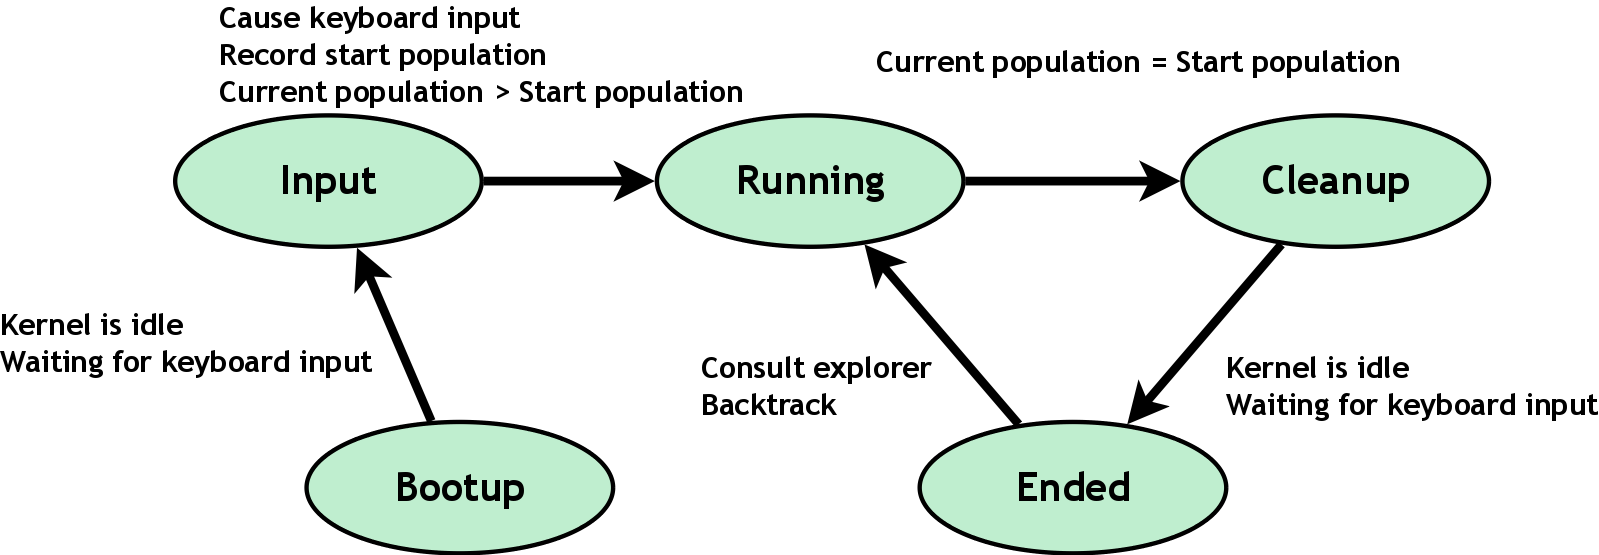
\includegraphics[width=0.8\textwidth]{teststate.png}
	\end{center}
	\caption{The test lifecycle state machine.}
	\label{fig:teststate}
\end{figure}
Landslide knows the state of the test case through a simple state machine, which is updated with information about the number of threads currently on the system, the number of threads on the runqueue, the state of the idle thread (if it exists), and whether or not the shell is waiting for keyboard input.

The state machine relies on certain information provided by the scheduler (Section~\ref{sec:components-sched}).

\begin{itemize}
	\item {\bf Is the shell waiting for keyboard input?} In general, the shell only waits for keyboard input when the kernel is ready for the user (or Landslide) to cause a test to run, or after the test has finished and a new one could be run.
		However, the shell may sometimes be waiting for keyboard input while other threads have some work to do (for example, the init process might not yet have reaped a reparented child process), and this work may be affected by race conditions during the test, so we need to include it in the test as well. For these cases an additional check is needed.
	\item {\bf Is the kernel idling?} This indicates whether any work is left to be done during bootup or during teardown.
	\item {\bf How many threads currently exist on the system?} This indicates whether the test has begun running.
\end{itemize}

The states in the test lifecycle, and the rules for transitioning between them, are as follows.

\begin{enumerate}
	\item {\bf Bootup.} Initial state. When the kernel is idling and the shell is waiting for keyboard input, advance state.
	\item {\bf Keyboard input.} Record the current thread count (the ``start population''). Generate keystrokes to cause the desired test case to run.
		When the current thread count is greater than the start population, advance state.
	\item {\bf Test running.} Begin constructing the decision tree here (since it is pointless to backtrack to before the test begins). When the current thread count equals the start population, advance state.
	\item {\bf Test cleanup.} The test processes have exited, but some housekeeping may yet remain. When the the kernel is idling and the shell is waiting for keyboard input, advance state.
	\item {\bf Test ended.} Invoke the explorer (Section~\ref{sec:components-explore}) to decide whom to rewind, and backtrack (to step 3).
\end{enumerate}

Figure~\ref{fig:teststate} depicts the states and transitions visually.

\section{Identifying Bugs}
\label{sec:techniques-bugs}

In order to identify when the guest kernel has done something incorrect, Landslide performs several different types of checks, some accurate but noncomprehensive, and some heuristic-based.

\subsection{Definite Bug-Detection Conditions}

\begin{enumerate}
	\item {\bf Kernel panic bugs.} If the kernel invoked \texttt{panic}, it detected its own bug, and Landslide need do nothing but report it.
	\item {\bf Use-after-free bugs.} Whenever the kernel accesses memory in the heap (when not in the dynamic allocator itself), Landslide verifies that the address is within an allocated range. If not, Landslide proclaims the access to be illegal.\footnote{In the same way, Landslide also detects calls to \texttt{free} on blocks that were already freed or never allocated at all.}
	\item {\bf Deadlock bugs.} If Landslide finds no runnable threads on the runqueue,\footnote{Except for idle, if it exists.} or if it detects a cycle of threads blocked on each other, it declares that the kernel has deadlocked.
\suspend{enumerate}

\subsection{Probable Bug-Detection Conditions}

\revision{
\begin{figure}[ht]
	\centering
	\begin{tabular}{cc}
	\subfloat[Infinite loop without decision points. Disproportionately many instructions have been executed since the red state, so the kernel is probably stuck in a ``tight'' loop.]{
	\hspace{0.12\textwidth}
	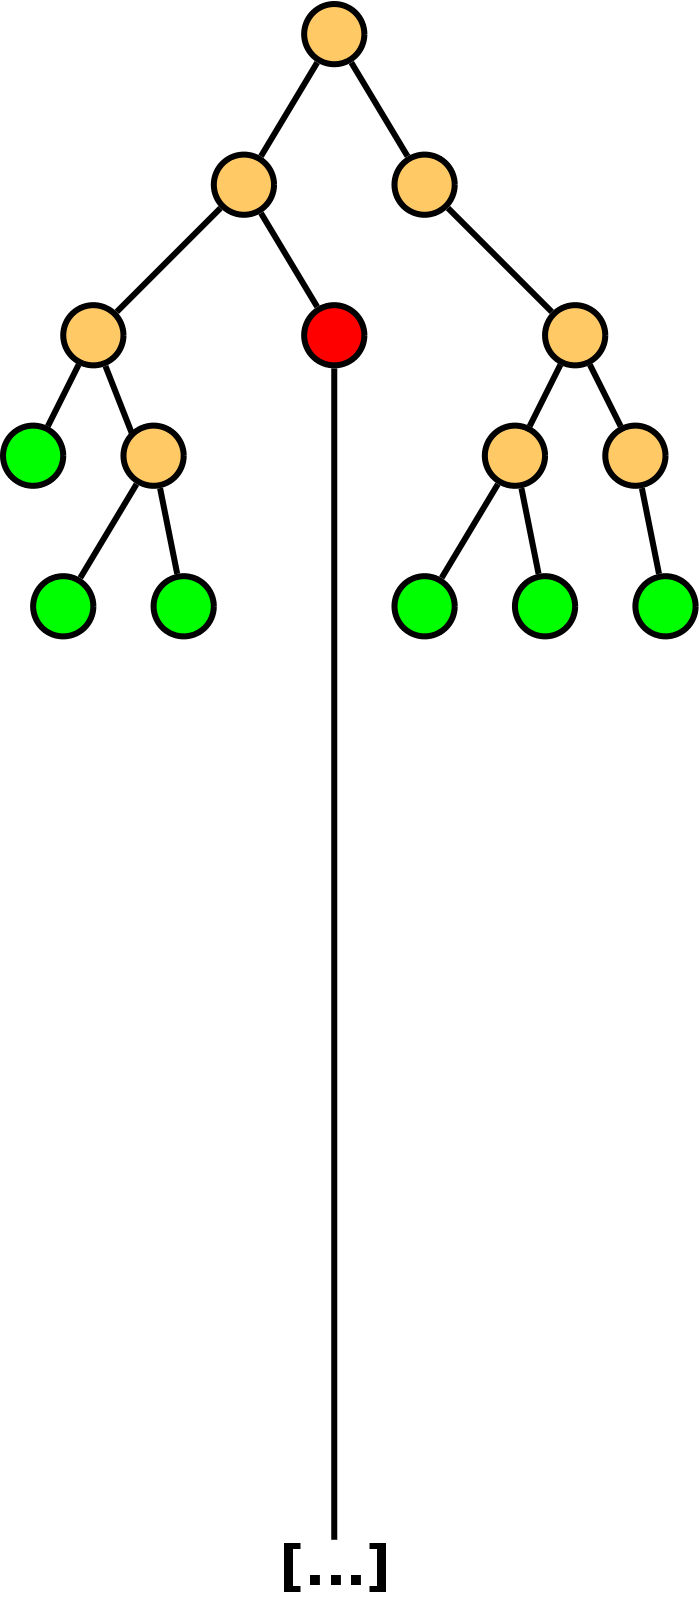
\includegraphics[width=0.2\textwidth]{tightloop.png}
	\hspace{0.12\textwidth}
	} &
	\subfloat[Infinite loop around decision points. Disproportionately many decision points have been encountered on the red branch, so the kernel is probably stuck in a loop around certain decision points.]{
	\hspace{0.12\textwidth}
	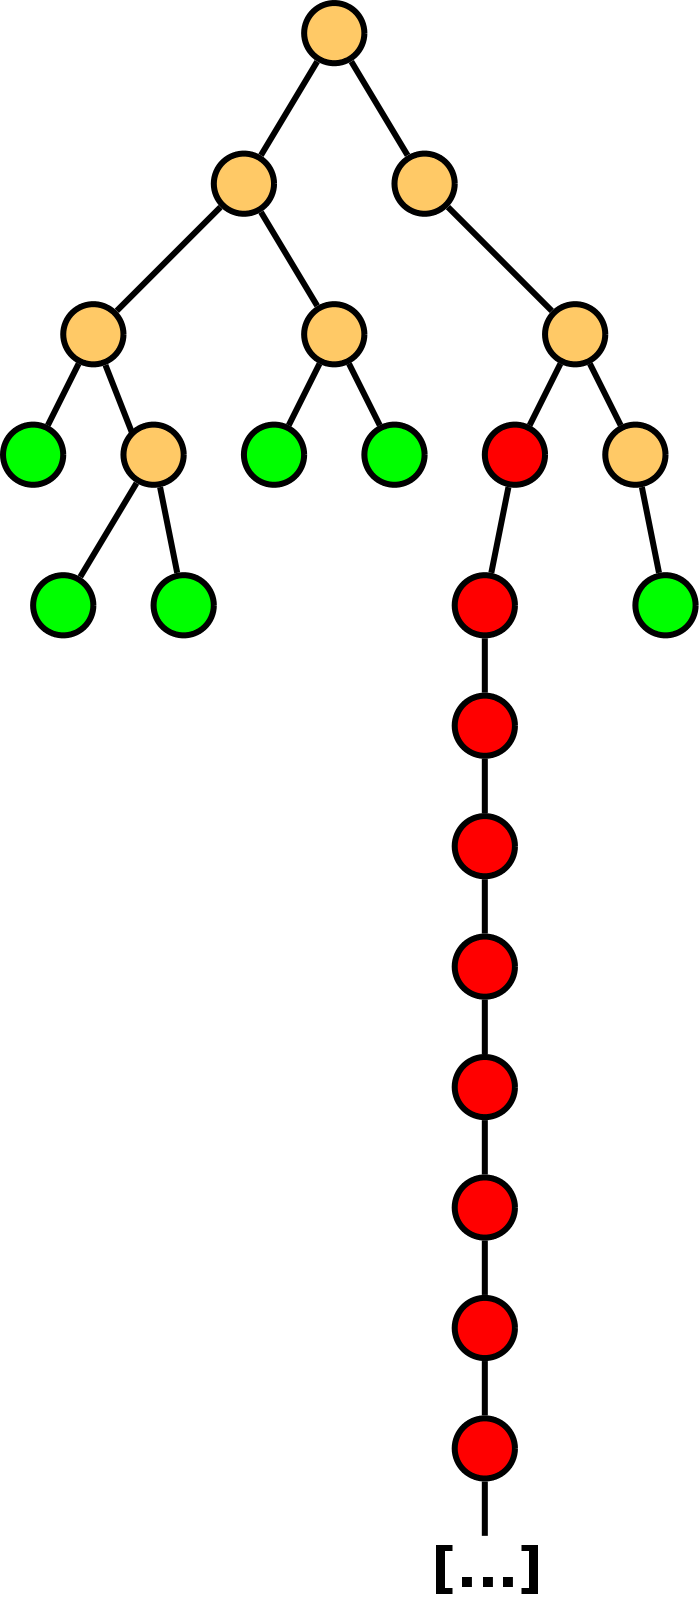
\includegraphics[width=0.2\textwidth]{livelock.png}
	\hspace{0.12\textwidth}
	}
	\end{tabular}
	\caption{Landslide judges whether the kernel has gotten stuck by analysing the structure of the execution tree. The red branches indicate non-terminating thread interleavings, which Landslide would identify by comparing them with other branches in their respective trees.}
	\label{fig:infiniteloop}
\end{figure}
}

\resume{enumerate}
	\item {\bf Memory leak bugs.} Landslide records the state of the heap before the test case begins, and compares it to the state of the heap after the test case ends. If memory allocated during the test was not freed, Landslide assumes that it was leaked.
		(Some kernel designs may legitimately behave this way, so this bug-check may be disabled when testing such kernels.)\footnote{There is, of course, much room for improvement in this metric, but it is not part of the research contribution.}
	\item {\bf Infinite loop bugs.} Landslide judges whether the kernel has entered an infinite loop by comparing the current branch of the decision tree to past executions of the same test case.
	Figure~\ref{fig:infiniteloop} depicts such tree structures in abstract.
	\begin{itemize}
		\item {\bf Infinite loops without decision points.} While exploring the decision tree, Landslide computes the average number of instructions executed between two consecutive decision points. If at any point the current number of instructions executed since the most recent decision point exceeds this average times a constant factor (arbitrarily chosen to be 2000), Landslide assumes the kernel must have gotten stuck in an infinite loop.
		\item {\bf Infinite loops around decision points.} Landslide also computes the average number of decision points in each branch of the decision tree (the average ``branch depth''). If the depth of the current branch ever exceeds this average times a constant factor (arbitrarily chosen to be 20), Landslide assumes the kernel must have gotten stuck in an infinite loop.
	\end{itemize}
	\revision{In our experience, these heuristics have never falsely identified an infinite loop when the kernel was making real progress.
	However, both of these heuristics require a minimum number of branches to be explored before Landslide considers the already-explored tree structure to be statistically significant (arbitrarily chosen to be 20).
	As such, these heuristics occasionally fail to trigger on a real infinite loop in cases when the loop occurs before enough ``safe'' branches were explored. In the future we might improve this heuristic by scaling the associated cutoff factor depending on how many branches were explored: the fewer branches explored so far, the less reliable the comparison, and hence the higher the cutoff factor to be used.}
\end{enumerate}

\section{Partial-Order Reduction}
\label{sec:techniques-por}

We make use of Dynamic Partial-Order Reduction (DPOR), the state-space pruning algorithm presented in \cite{dpor}. DPOR requires two sets to be computed that describe the concurrency relationship between transitions: the happens-before relation, and the memory independence relation. Here we discuss the specifics of implementing these in our environment.

\subsection{Happens-Before Relation}

\revision{The happens-before relation expresses for each pair of transitions whether executing the first one is required to ``enable'' the second one. In order to establish the relation,} Landslide uses the state of the scheduler runqueues (Section~\ref{sec:components-sched}), which are snapshotted at every decision point (Section~\ref{sec:components-explore}).

Unfortunately, a thread's presence or absence on the scheduler runqueue does not necessarily correspond to whether it is {\em runnable} at any point. We identify three exceptions, as foreshadowed in Section~\ref{sec:challenges-design}:

\begin{itemize}
	\item {\bf Current thread not on runqueue.} If the currently-running thread is not stored on the runqueue, we identify it as runnable anyway (except in the special case of idle, as described below).
	\item {\bf Idle thread.} Some kernels may have an explicit idle thread and store it on the runqueue, with explicit code to skip over it if other threads are runnable. Hence, if the idle thread is on the runqueue (and/or the current thread), it is only runnable if no other threads are runnable.
	\item {\bf Yielding mutexes.} In kernels whose mutexes (or other synchronisation idioms) leave threads on the runqueue when they are notionally blocked, Landslide classifies such threads as not runnable.
\end{itemize}

Using this notion of runnability, the happens-before relation is established as follows. Let $X$ be a transition and $Y$ be a subsequent transition in a branch that was just explored, and $T_Y$ be the thread associated with $Y$. We say that $X$ {\em enables} $Y$ if $T_Y$ was not runnable immediately before $X$, but was runnable immediately after. Then, a transition $A$ happens-before a transition $B$ if $T_A$ is the same thread as $T_B$, if $A$ enables $B$, or if $A$ happens-before some transition $C$ that enables $B$.

\subsection{Memory Independence Relation}
\label{sec:por-independence}
The independence relation expresses which transitions do not read-and-write or write-and-write to the same shared memory addresses. Landslide computes this relation using the set of shared memory accesses described in Section~\ref{sec:components-memory}. We encountered two challenges pertaining to memory independence:

\begin{itemize}
	\item {\bf Always-accessed memory locations.}
		In kernel-space, every thread switch goes through common scheduler and context-switcher routines. These routines inevitably access scheduler data structures, such as the runqueue. The timer tick counter is another example: this global variable is not necessarily accessed every transition, because voluntary reschedules do not involve timer interrupts, but every involuntary preemption will cause a write to this counter.

		If we include such memory accesses in the independence relation, it will result that all transitions conflict, and DPOR won't be able to achieve any reduction. To allow for state space reduction, we sacrifice our ability to find races involving these particular accesses by ignoring them. Currently we require the user to identify these locations as part of the instrumentation process, as described in Section~\ref{sec:using-config-landslide}.
	\item {\bf Freed memory poisoning.}
		A use-after-free bug happens whenever one thread accesses an address within an allocated block that another thread previously freed. Even if no other code makes a conflicting access to the same address after the \texttt{free}, accessing dynamically-allocated memory after it has been freed is illegal no matter what.

		Hence, even if the second thread that freed the block never accesses the particular address that the first thread used, the second thread's \texttt{free} still logically conflicts with the first thread's access. Landslide addresses this by treating every call to \texttt{free} as a {\em write} access to every address within the freed block when computing shared memory conflicts.
\end{itemize}

\subsection{Soundness}

\revision{
Because we recommend using Landslide with coarse-grained decision sets, as opposed to mandating a decision point between every pair of shared memory accesses, it is possible for Landslide to overlook race conditions that require finer-grained interleavings to expose. In this way, Landslide's search is not ``sound'', but instead false-negative-oriented.

We do, however, claim that Landslide's search is sound in a different way: if the provided decision points are sufficient to express an interleaving that would expose a race, then Landslide will find it. That is, if Landslide is exploring an execution tree with bugs in some branches, it will eventually find a bug.

Dynamic Partial Order Reduction works by identifying ``evil ancestors'' for each transition in a branch after executing that branch. Intuitively, a transition's evil ancestor is another transition such that executing the test with the order of those two transitions reversed could cause different concurrent behaviour to arise.}
\cite{dpor} and \cite{dbug-retreat} present a partial order reduction algorithm in which only the first evil ancestor of each transition need be considered when identifying which alternate interleavings need to be explored.

\begin{figure}[h]
	\centering
	\begin{tabular}{cc}
	\subfloat[Race-free interleaving.]{
		\footnotesize
		\begin{tabular}{l|c|c|c|}
			\cline{2-4}
			& {\bf Thread 1} & {\bf Thread 2} & {\bf Thread 3} \\
			\cline{2-4}
			$A$ & \texttt{x=42;} & & \\
			$B$ & & \texttt{y=31337;} & \\
			\multirow{2}{*}{$C_1$} & & & \texttt{if (y==31337)} \\
			& & & \texttt{assert(x==42);} \\
			\cline{2-4}
		\end{tabular}
	} &
	\subfloat[Alternate interleaving explored with DPOR.]{
		\footnotesize
		\begin{tabular}{l|c|c|c|}
			\cline{2-4}
			& {\bf Thread 1} & {\bf Thread 2} & {\bf Thread 3} \\
			\cline{2-4}
			$A$ & \texttt{x=42;} & & \\
			$C_2$ & & & \texttt{if (y==31337)} \\
			$B$ & & \texttt{y=31337;} & \\
			\cline{2-4}
		\end{tabular}
	} \\
	\multicolumn{2}{c}{
	\subfloat[Buggy interleaving.]{
		\footnotesize
		\begin{tabular}{l|c|c|c|}
			\cline{2-4}
			& {\bf Thread 1} & {\bf Thread 2} & {\bf Thread 3} \\
			\cline{2-4}
			$B$ & & \texttt{y=31337;} & \\
			\multirow{2}{*}{$C_3$} & & & \texttt{if (y==31337)} \\
			& & & \texttt{assert(x==42);} \\
			$A$ & \texttt{x=42;} & & \\
			\cline{2-4}
		\end{tabular}
	}}
	\end{tabular}
	\caption{This sample code defeats a DPOR implementation that uses only the first evil ancestor if a decision point is not defined between the two lines of thread 3's code. The first interleaving is explored first; DPOR identifies transition $B$ as the first evil ancestor of $C_1$, and runs the second interleaving next, reordering them. In the second interleaving, $A$ is no longer a second evil ancestor of $C_2$, so the third interleaving is never explored, and the assertion failure is missed.}
	\label{fig:evil-ancestors}
\end{figure}

We found that implementing DPOR in this way violated our second notion of soundness, because it relies on the invariant that each transition contains only one inter-thread communication event (in kernel-space, this means a shared memory access).
\revision{However, a key point of Landslide's recommended usage pattern is to sacrifice maximally-fine-grained decision points for performance, and so multiple different shared memory conflicts may happen in each transition.} Figure~\ref{fig:evil-ancestors} demonstrates a counterexample to the soundness of identifying only one evil ancestor per transition given our usage pattern.

\revision{Instead, Landslide uses considers every evil ancestor of each transition when performing DPOR. This modification enables Landslide to avoid the problem presented in the figure, because it will identify both alternate interleavings after exploring the first one. We claim without certainty that this change restores the second notion of soundness to Landslide's search, and leave proving this property to future work.}

\section{Debugging Feedback}
\label{sec:techniques-feedback}

\begin{figure}[h]
	%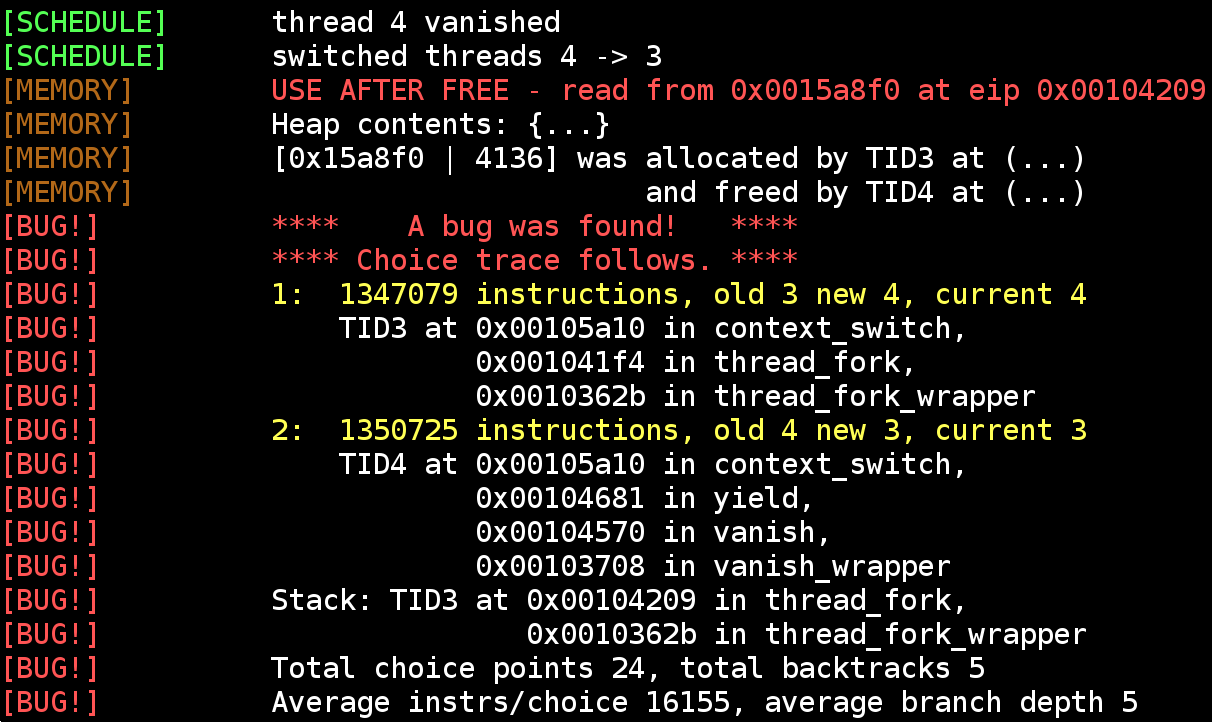
\includegraphics[width=0.95\textwidth]{found_a_bug.png}
	\centering
	\colorbox{black}{\color{white}
	{\small
	\begin{tabular}{l}
	\texttt{\hilight{green}{[SCHEDULE]}~~~~~~thread 4 vanished} \\
	\texttt{\hilight{green}{[SCHEDULE]}~~~~~~switched threads 4 -> 3} \\
	\texttt{\hilight{brown}{[MEMORY]}~~~~~~~~\hilight{red}{USE AFTER FREE - read from 0x0015a8f0 at eip 0x00104209}} \\
	\texttt{\hilight{brown}{[MEMORY]}~~~~~~~~Heap contents:~\{...\}} \\
	\texttt{\hilight{brown}{[MEMORY]}~~~~~~~~[0x15a8f0 | 4136] was allocated by TID3 at (...)} \\
	\texttt{\hilight{brown}{[MEMORY]}~~~~~~~~~~~~~~~~~~~~~~~~~~~~~~and freed by TID4 at (...)} \\
	\texttt{\hilight{red}{[BUG!]}~~~~~~~~~~\hilight{red}{****~~~~~A bug was found!~~~~****}} \\
	\texttt{\hilight{red}{[BUG!]}~~~~~~~~~~\hilight{red}{**** Decision trace follows.~****}} \\
	\texttt{\hilight{red}{[BUG!]}~~~~~~~~~~\hilight{yellow}{1:~~1347079 instructions, old 3 new 4, current 4}} \\
	\texttt{\hilight{red}{[BUG!]}~~~~~~~~~~~~~~TID3 at 0x00105a10 in \hilight{cyan}{context\_switch},} \\
	\texttt{\hilight{red}{[BUG!]}~~~~~~~~~~~~~~~~~~~~~~0x001041f4 in \hilight{cyan}{thread\_fork},} \\
	\texttt{\hilight{red}{[BUG!]}~~~~~~~~~~~~~~~~~~~~~~0x0010362b in \hilight{cyan}{thread\_fork\_wrapper}} \\
	\texttt{\hilight{red}{[BUG!]}~~~~~~~~~~\hilight{yellow}{2:~~1350725 instructions, old 4 new 3, current 3}} \\
	\texttt{\hilight{red}{[BUG!]}~~~~~~~~~~~~~~TID4 at 0x00105a10 in \hilight{cyan}{context\_switch},} \\
	\texttt{\hilight{red}{[BUG!]}~~~~~~~~~~~~~~~~~~~~~~0x00104681 in \hilight{cyan}{yield},} \\
	\texttt{\hilight{red}{[BUG!]}~~~~~~~~~~~~~~~~~~~~~~0x00104570 in \hilight{cyan}{vanish},} \\
	\texttt{\hilight{red}{[BUG!]}~~~~~~~~~~~~~~~~~~~~~~0x00103708 in \hilight{cyan}{vanish\_wrapper}} \\
	\texttt{\hilight{red}{[BUG!]}~~~~~~~~~~Stack:~TID3 at 0x00104209 in \hilight{cyan}{thread\_fork},} \\
	\texttt{\hilight{red}{[BUG!]}~~~~~~~~~~~~~~~~~~~~~~~~~0x0010362b in \hilight{cyan}{thread\_fork\_wrapper}} \\
	\texttt{\hilight{red}{[BUG!]}~~~~~~~~~~Total decision points 24, total backtracks 5} \\
	\texttt{\hilight{red}{[BUG!]}~~~~~~~~~~Average instrs/decision 16155, average branch depth 5} \\
	\end{tabular}
	}
	}
	\caption{A sample decision trace (with extraneous text trimmed) that Landslide generated using the \texttt{double\_thread\_fork} test case (Section~\ref{sec:using-tests}).}
	\label{fig:found_a_bug}
\end{figure}

In its unique position of control over when the kernel gets preempted and which thread gets scheduled at each context switch, Landslide has the capability to provide the user with detailed information about a test case's execution.
When Landslide determines that a bug was found, it immediately aborts exploration of the decision tree, and prints a {\em decision trace}: a comprehensive report of the particular interleaving of thread transitions that caused the bug to appear. Figure~\ref{fig:found_a_bug} depicts a simple decision trace for a use-after-free bug.

The decision trace explains each preemption or voluntary reschedule in the interleaving: which thread used to be running, which thread was chosen to run instead, and the stack trace of the former thread at the point from which it was switched away.

Landslide also prints the stack trace of the currently-running thread at the point where the bug was found, and (optionally) drops the user into the Simics debugging prompt. Depending on the nature of the bug found, Landslide also provides more detailed information:

\begin{enumerate}
	\item If the kernel has panicked, Landslide prints the message used in the panic/assertion.
	\item If a use-after-free bug is found, Landslide prints information about the most-recently-freed chunk containing the accessed address: the stack trace and TID both for when it was allocated and freed.
	\item If deadlock is detected, Landslide prints the cycle of TIDs that are blocked on each other.\footnote{This currently only works when using the annotations for yielding mutexes, though it is not difficult to implement more generally.}
	\item If a memory leak is suspected, Landslide prints how many bytes bigger the heap is after the test ended than when the test began.\footnote{Future feature: Printing when-allocated stack traces for each suspicious heap chunk.}
	\item If an infinite loop is suspected, depending on which heuristic was triggered, Landslide prints either the number of instructions since the last decision point (and the previous average) or the current branch depth (and the previous average).
\end{enumerate}

Landslide can also provide other useful information, even in cases where it did not find bugs, to help with the user's process of configuring decision points. Instead of exploring alternative interleavings, it can stop execution after the first interleaving and print out the set of decision points that were identified, along with the shared memory conflicts and happens-before relations for pairs of transitions between the decision points.
